\documentclass[11pt]{article}
\usepackage{enumitem}
\usepackage[margin=1in]{geometry}
\usepackage{graphicx}
\usepackage[space]{grffile}
\usepackage{adjustbox}
\usepackage{indentfirst}
\usepackage{amsmath}
\usepackage{physics}
\usepackage{tabu}
\usepackage{color}

\title{\textbf{CSM146 Homework 2}}
\author{Zipeng Fu}
\date{\today}

\begin{document}
\maketitle
\newpage 

\section{Perceptron}
    Let the 2 inputs to be $x_1$ and $x_2$, whose values are 1 for ture and -1 for false, then the feature vector is $X = (1\;x_1\;x_2)$. Let the classifier $\Theta = (\theta_0\;\theta_1\;\theta_2)$. The linear threshold units classify an example, represented as feature vector $X$, by output = sgn($\Theta^TX$).
\begin{enumerate}[label=(\alph*)]
\item
    $\Theta_1 = (-0.5\;1\;1)$, $\Theta_2 = (-1.5\;2\;1)$
\item
    There is no perceptron/linear classifier that can separate all 4 instances of XOR operation, an example of the parity function. ``False'' output is in 1st and 3rd quodrant and ``True'' output is in 2nd and 4th quodrant. Hence, no single line is the decision boundary.
\end{enumerate}


\section{Logistic Regression}
\begin{enumerate}[label=(\alph*)]
\item
    $$J(\theta) = \sum^N_{n=1}{\left[y_n\text{log}\left(1+e^{-\theta^Tx_n}\right)+(1-y_n)\text{log}\left(1+e^{\theta^Tx_n}\right)\right]}$$
    \begin{equation*}
    \begin{split}
        \pdv{J}{\theta_j}
        & = \sum^N_{n=1}{\left[y_n\left(1+e^{-\theta^Tx_n}\right)^{-1}\left(e^{-\theta^Tx_n}\right)(-x_{nj})+(1-y_n)\left(1+e^{\theta^Tx_n}\right)^{-1}\left(e^{\theta^Tx_n}\right)x_{nj}\right]}\\
        & = \sum^N_{n=1}{\left[y_n\left(1+e^{\theta^Tx_n}\right)(-x_{nj})+(1-y_n)\left(1+e^{-\theta^Tx_n}\right)x_{nj}\right]}
    \end{split}
    \end{equation*}
\end{enumerate}


\section{Locally Weighted Linear Regression}
\begin{enumerate}[label=(\alph*)]
\item
    $$\pdv{J}{\theta_0} = \sum^N_{n=1}{2w_n\left(\theta_0+\theta_1x_{n,1}-y_n\right)}$$
    $$\pdv{J}{\theta_1} = \sum^N_{n=1}{2w_n x_{n,1}\left(\theta_0+\theta_1x_{n,1}-y_n\right)}$$
\item
    If $\pdv{J}{\theta_0}$ and $\pdv{J}{\theta_1}$ equal 0, then
    $$\left(\sum^N_{n=1}{w_n}\right)\theta_0 + \left(\sum^N_{n=1}{w_n x_{n,1}}\right)\theta_1 = \sum^N_{n=1}{w_n y_n},$$
    $$\left(\sum^N_{n=1}{w_n x_{n,1}}\right)\theta_0 + \left(\sum^N_{n=1}{w_n x_{n,1}^2}\right)\theta_1 = \sum^N_{n=1}{w_n x_{n,1} y_n}.$$
    Let $A = \sum^N_{n=1}{w_n}$, $B = \sum^N_{n=1}{w_n x_{n,1}}$, $C = \sum^N_{n=1}{w_n y_n}$, $D = \sum^N_{n=1}{w_n x_{n,1}}$, $E = \sum^N_{n=1}{w_n x_{n,1}^2}$, $F = \sum^N_{n=1}{w_n x_{n,1} y_n}$, then
    $
    \left(\begin{array}{@{}cc|c@{}}
        A & B & C\\
        D & E & F
    \end{array}\right)
    $
    is the matrix representation of these 2 equations. By Cramer's Rule,
    $$\theta_0 = \frac{\mathrm{det}\left(A_0\right)}{\mathrm{det}\left(A\right)} = \frac{CE-BF}{AE-BD},$$
    $$\theta_1 = \frac{\mathrm{det}\left(A_1\right)}{\mathrm{det}\left(A\right)} = \frac{AF-CD}{AE-BD}.$$
    Substitute $A, B, C, D, E, F$ and then the closed-formed solutions can be found.
\end{enumerate}


\section{Understanding Linear Separability}
\begin{enumerate}[label=(\alph*)]
\item
    If $D$ is linearly separable, there is still the case that $\vec{w}^T\vec{x_i} + \theta = 0$, which means that the end points of feature vectors of some samples may lie on the hyperplane. Let $\tilde{\theta} = \theta + \epsilon$, where $\epsilon > 0$ and is a infinitesimal number close to 0 so that the hyperplane is shifted/translated with minimal amount towards the negative half space, where $\vec{w}^T\vec{x_i} + \theta < 0$, and no feature points are on the hyperplane. Then $\forall (\vec{x_i}, y_i) \in D,\; \exists\vec{w}$, such that $y_i(\vec{w}^T\vec{x_i} + \tilde{\theta}) > 0$. In order for $\delta = 0$, we can simply increase the length of $\vec{w}$ and keep its direction unchanged. This is the process to normalize $\vec{w}$ without sufficient length. Hence, $y_i(\vec{w}^T\vec{x_i} + \tilde{\theta})$ will increase and eventually $y_i(\vec{w}^T\vec{x_i} + \tilde{\theta}) \geq 1$ for all examples.

\item
    If $\delta = 0$, then $\forall (\vec{x_i}, y_i) \in D$, $y_i(\vec{w}^T\vec{x_i} + \theta) \geq 1 \geq 0$. By the parity theory, either $\vec{w}^T\vec{x_i} + \theta \geq 0$ and $y_i \geq 0$ (ie. $y_i = 1$), or $\vec{w}^T\vec{x_i} + \theta < 0$ and $y_i < 0$ (ie. $y_i = -1$). This is equivalent to the condition (1). Hence, $D$ is linearly separable.

\item
    If $\delta \in (0, 1]$, then $y_i(\vec{w}^T\vec{x_i} + \theta) \in [0,1)$. By the parity theory, either $\vec{w}^T\vec{x_i} + \theta > 0$ and $y_i > 0$ (ie. $y_i = 1$), or $\vec{w}^T\vec{x_i} + \theta < 0$ and $y_i < 0$ (ie. $y_i = -1$). This satisfies the condition (1). Hence, $D$ is linearly separable in this case.

    If $\delta > 1$, then $\forall (\vec{x_i}, y_i) \in D$, $y_i(\vec{w}^T\vec{x_i} + \theta)$ is larger than a negative number, which means that $(\vec{w}^T\vec{x_i} + \theta)$ and $y_i$ can be with different signs. This does not satisfies the condition (1). Thus, in this case, the linear separability cannot be concluded.

\item
    The minimum $\delta$ is 0, with $y_i(\vec{w}^T\vec{x_i} + \theta) \geq 0$. Although, by the argument in (b), the condition (a) of linear separability is satisfied, it is possible for feature points to be on the hyperplane. As a result, it's not the optimal case where, by the argument in (a), no points are on the hyperplane with $\forall (\vec{x_i}, y_i) \in D$, $y_i(\vec{w}^T\vec{x_i} + \theta) > 0$, which is constructable given a linearly separable dataset $D$.

\item
    There are only 2 distinct sample points in the space, so the data set is definitely separable, with the minimum $\delta = 0$.
    Solution 1: $\delta = 0$, $\vec{w} = [1\quad1\quad1]^T$ and $\theta = 0$;\\
    Solution 2: $\delta = 0$, $\vec{w} = [1\quad0\quad0]^T$ and $\theta = 0$;\\
    Solution 3: $\delta = 0$, $\vec{w} = [0\quad1\quad0]^T$ and $\theta = 0$;\\
    ...\\
    Any hyperplane exists between the end points of $\vec{x_1}$ and $\vec{x_2}$ will give optimal solutions where $\delta = 0$. Pick the normal vector of the hyperplane, $\vec{w}$, to be sufficiently large so that  $y_i(\vec{w}^T\vec{x_i} + \tilde{\theta}) \geq 1$ for both examples.\\\\
    General solution:
    $$w_1 + ... + w_n + \theta \geq 1 \quad\text{and}\quad -w_1 - ... - w_n + \theta \leq -1.$$
    $$\text{So, } w_1 + ... + w_n \geq |\theta| + 1.$$


\end{enumerate}


\section{Implementation: Polynomial Regression}
\begin{enumerate}[label=(\alph*)]
\item
    \adjustbox{valign=t}{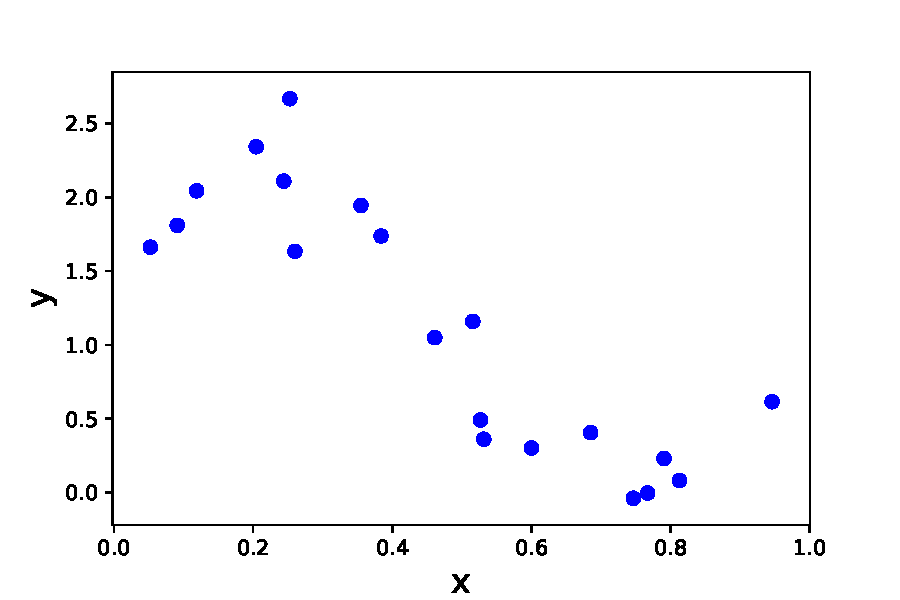
\includegraphics[width=0.5\textwidth]{regression_train.pdf}}
    \adjustbox{valign=t}{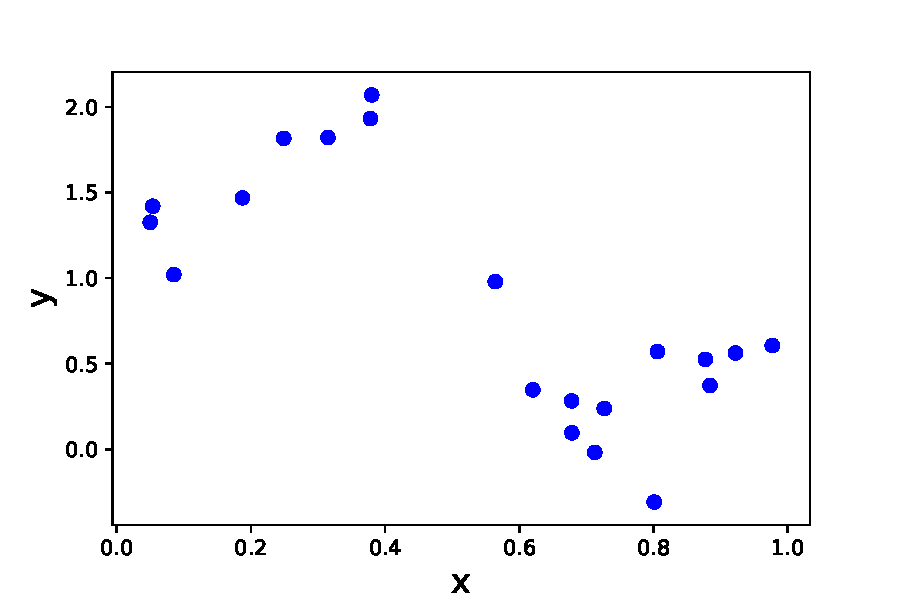
\includegraphics[width=0.5\textwidth]{regression_test.pdf}}\\\\
    The variance of the data is relatively large. The graph of training set on the left side generally shows a trend in negative correlation if we apply the linear regression model. However, the test set may not be suitable for linear regression, because data behave like gathering in 2 parts.

\item 
    Done. (Code in Appendix)

\item 
    Done. (Code in Appendix)

\item 
    If we set the coefficent vector to be zero vector, the cost will be 40.233847409671.\\\\
    For different learning rate, we get the following table,\\
    \begin{center}
        \begin{tabular}{||c c c c||} 
        \hline
        learning rate $\eta$ & iterations & final value of $J(\theta)$ & time taken\\ [0.5ex] 
        \hline\hline
        0.0407 & 10000 & 2.71091652001e+39 & 0.19749999046325684 \\ 
        \hline
        0.01 & 765 & 3.91257640579 & 0.023038148880004883\\
        \hline
        0.001 & 7021 & 3.91257640579 & 0.16843152046203613\\
        \hline
        0.0001 & 10000 & 4.0863970368 & 0.2326192855834961\\ [1ex]
        \hline
       \end{tabular}
    \end{center}

    \textbf{\textcolor{red}{NOTE}}: My $fit\_GD$ first calculates the the error of the initial 0 coefficent vector, put it into $err\_list$, and then do the gradient computation. Hence, if the implementation is first calcuating the gradient, the final counts of iteration for $\eta = 0.01\;\text{or}\;0.001$ will have 1 more iteration, 766 and 7022 respectively.

    When the learning rate is too large, in the case of $\eta = 0.0407$, the objective function will not converge and the value will oscillate and diverge to produce a large error. In contrast, when the learning rate is too small, in the case of $\eta = 0.0001$, the value of objective function does not converge before reaching the 10000th iteration. As we can see, the final error over the training set, in term of objective function, is 3.91257640579. And the resulting coefficent vector for $\eta = 0.01$ is [2.44640703 -2.81635347] and the one for $\eta = 0.001$ is [2.4464068 -2.816353]. Since the objective function is convex, there should be no difference in the optimal coefficent vector theoretically. I think the discrepency is due to floating point precision lost during different procedures the gradient descent follows.

\item 
    The coefficent vector is [2.44640709 -2.81635359], which is the same with global minimum abtained in part (d) if the floating-point precision lost is taken into account. The time taken is 0.0010113716125488281, which is much faster than the open-loop $fit\_GD$ method.\\

\item 
    \begin{verbatim}
Investigating varied eta (start with k=1)...
number of iterations: 616
time taken:  0.018046855926513672
model cost:  3.91257640579
coefficent vector: [ 2.44640732 -2.81635404]
    \end{verbatim}
    \begin{verbatim}
Investigating varied eta (start with k=0)...
number of iterations: 1679
time taken:  0.05411362648010254
model cost:  3.91257640579
coefficent vector: [ 2.44640678 -2.81635296]
    \end{verbatim}

\item 
    Done. (Code in Appendix)

\item 
    Implementation of $rms\_error$ is shown in Appendix.\\\\
    RMSE method includes a normalizaton term $N$ and the square root alleviates the enlarged distance $(h_\theta(x_n)-y_n)^2$ between the expected $y$, calculated by $h_\theta(x_n)$, and the actual $y_n$. Thus, RMSE acts like the standard deviation of actual data from the predictions, but 

\item
    \adjustbox{valign=t}{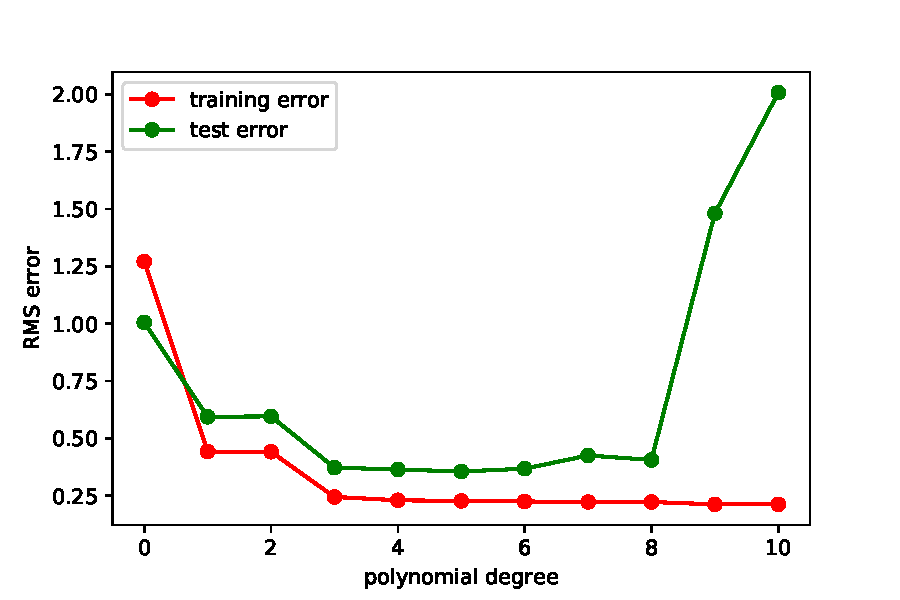
\includegraphics{degree.pdf}}\\
    The best fit on training data is the 10th order polynomial ($m$=10) with training error: 0.211689163163471, test error: 2.0077034764205193. \\\\
    With the limited size of training set and test set, I will rely on the test error to pick the degree polynomial that best fits the whole data set. The minimum test error is 0.3551377428840611 with degree 5 and training error 0.22681133051783212. Notice that the training error in this case is also very close to the best training error, with a difference of 0.015.\\\\
    Underfitting occurs when degree $\leq$ 2, where the training error is at least 2 times as high as the RMS training error rate of $m \geq 2$. Overfitting happens when degree $geq$ 8, where from $m = 8$ to $m = 9$, the training error rate keeps decreasing but the test error jumps to more than 3 times of its original rate.

\end{enumerate}
\newpage

\section*{Appendix: regression.py}
\begin{verbatim}
# This code was adapted from course material by Jenna Wiens (UMichigan).

# python libraries
import os

# numpy libraries
import numpy as np

# matplotlib libraries
import matplotlib as mpl
import matplotlib.pyplot as plt

import time

######################################################################
# classes
######################################################################

class Data :
    
    def __init__(self, X=None, y=None) :
        """
        Data class.
        
        Attributes
        --------------------
            X       -- numpy array of shape (n,d), features
            y       -- numpy array of shape (n,), targets
        """
        
        # n = number of examples, d = dimensionality
        self.X = X
        self.y = y
    
    def load(self, filename) :
        """
        Load csv file into X array of features and y array of labels.
        
        Parameters
        --------------------
            filename -- string, filename
        """
        self.filename = filename

        # determine filename
        dir = os.path.dirname('__file__')
        f = os.path.join(dir, 'data', filename)
        
        # load data
        with open(f, 'r') as fid :
            data = np.loadtxt(fid, delimiter=",")
        
        # separate features and labels
        self.X = data[:,:-1]
        self.y = data[:,-1]
    
    def plot(self, **kwargs) :
        """Plot data."""
        
        if 'color' not in kwargs :
            kwargs['color'] = 'b'
        
        plt.scatter(self.X, self.y, **kwargs)
        plt.xlabel('x', fontsize = 16)
        plt.ylabel('y', fontsize = 16)
        #plt.savefig('{}.pdf'.format(self.filename))
        plt.show()

# wrapper functions around Data class
def load_data(filename) :
    data = Data()
    data.load(filename)
    return data

def plot_data(X, y, **kwargs) :
    data = Data(X, y)
    data.plot(**kwargs)


class PolynomialRegression() :
    
    def __init__(self, m=1, reg_param=0) :
        """
        Ordinary least squares regression.
        
        Attributes
        --------------------
            coef_   -- numpy array of shape (d,)
                        estimated coefficients for the linear regression problem
            m_      -- integer
                        order for polynomial regression
            lambda_ -- float
                        regularization parameter
        """
        self.coef_ = None
        self.m_ = m
        self.lambda_ = reg_param
    
    
    def generate_polynomial_features(self, X) :
        """
        Maps X to an mth degree feature vector e.g. [1, X, X^2, ..., X^m].
        
        Parameters
        --------------------
            X       -- numpy array of shape (n,1), features
        
        Returns
        --------------------
            Phi     -- numpy array of shape (n,(m+1)), mapped features
        """
        
        n,d = X.shape
        
        ### ========== TODO : START ========== ###
        # part b: modify to create matrix for simple linear model
        # part g: modify to create matrix for polynomial model
        m = self.m_
        if d == m+1:
            Phi = X
        else:
            Phi = np.ones((n, 1), dtype = int)
            for i in range(m):
                Phi = np.column_stack((Phi, X**(i+1)))
        
        ### ========== TODO : END ========== ###
        
        return Phi
    
    
    def fit_GD(self, X, y, eta=None,
                eps=0, tmax=10000, verbose=False) :
        """
        Finds the coefficients of a {d-1}^th degree polynomial
        that fits the data using least squares batch gradient descent.
        
        Parameters
        --------------------
            X       -- numpy array of shape (n,d), features
            y       -- numpy array of shape (n,), targets
            eta     -- float, step size
            eps     -- float, convergence criterion
            tmax    -- integer, maximum number of iterations
            verbose -- boolean, for debugging purposes
        
        Returns
        --------------------
            self    -- an instance of self
        """
        if self.lambda_ != 0 :
            raise Exception("GD with regularization not implemented")
        
        if verbose :
            plt.subplot(1, 2, 2)
            plt.xlabel('iteration')
            plt.ylabel(r'$J(\theta)$')
            plt.ion()
            plt.show()
        
        X = self.generate_polynomial_features(X) # map features
        n,d = X.shape
        eta_input = eta
        self.coef_ = np.zeros(d)                 # coefficients
        err_list  = np.zeros((tmax,1))           # errors per iteration
        
        # GD loop
        for t in range(tmax) :
            ### ========== TODO : START ========== ###
            # part f: update step size
            # change the default eta in the function signature to 'eta=None'
            # and update the line below to your learning rate function
            if eta_input is None :
                eta = 1/(1+t)
            else :
                eta = eta_input
            ### ========== TODO : END ========== ###
                
            ### ========== TODO : START ========== ###
            # part d: update theta (self.coef_) using one step of GD
            # hint: you can write simultaneously update all theta using vector math
                
            # track error
            # hint: you cannot use self.predict(...) to make the predictions
            y_pred = self.predict(X)
            err_list[t] = np.sum(np.power(y - y_pred, 2)) / float(n)
            self.coef_ -= 2*eta*np.dot(X.T, (y_pred-y))
            ### ========== TODO : END ========== ###
            
            # stop?
            if t > 0 and abs(err_list[t] - err_list[t-1]) <= eps :
                break
            
            # debugging
            if verbose :
                x = np.reshape(X[:,1], (n,1))
                cost = self.cost(x,y)
                plt.subplot(1, 2, 1)
                plt.cla()
                plot_data(x, y)
                self.plot_regression()
                plt.subplot(1, 2, 2)
                plt.plot([t+1], [cost], 'bo')
                plt.suptitle('iteration: %d, cost: %f' % (t+1, cost))
                plt.draw()
                plt.pause(0.05) # pause for 0.05 sec
        
        print('number of iterations: %d' % (t+1))
        
        return self
    
    
    def fit(self, X, y, l2regularize = None ) :
        """
        Finds the coefficients of a {d-1}^th degree polynomial
        that fits the data using the closed form solution.
        
        Parameters
        --------------------
            X       -- numpy array of shape (n,d), features
            y       -- numpy array of shape (n,), targets
            l2regularize    -- set to None for no regularization. set to positive double for L2 regularization
                
        Returns
        --------------------        
            self    -- an instance of self
        """
        
        X = self.generate_polynomial_features(X) # map features
        
        ### ========== TODO : START ========== ###
        # part e: implement closed-form solution
        # hint: use np.dot(...) and np.linalg.pinv(...)
        #       be sure to update self.coef_ with your solution
        invX = X.T
        self.coef_ = np.linalg.pinv(np.dot(invX, X)).dot(invX).dot(y)
        
        ### ========== TODO : END ========== ###
    
    
    def predict(self, X) :
        """
        Predict output for X.
        
        Parameters
        --------------------
            X       -- numpy array of shape (n,d), features
        
        Returns
        --------------------
            y       -- numpy array of shape (n,), predictions
        """
        if self.coef_ is None :
            raise Exception("Model not initialized. Perform a fit first.")
        
        X = self.generate_polynomial_features(X) # map features
        
        ### ========== TODO : START ========== ###
        # part c: predict y
        y = np.dot(X, self.coef_)
        ### ========== TODO : END ========== ###
        
        return y
    
    
    def cost(self, X, y) :
        """
        Calculates the objective function.
        
        Parameters
        --------------------
            X       -- numpy array of shape (n,d), features
            y       -- numpy array of shape (n,), targets
        
        Returns
        --------------------
            cost    -- float, objective J(theta)
        """
        ### ========== TODO : START ========== ###
        # part d: compute J(theta)
        if self.coef_ is None :
            raise Exception("Model not initialized. Perform a fit first.")
        X = self.generate_polynomial_features(X)
        cost = ((np.dot(X, self.coef_) - y)**2).sum()
        ### ========== TODO : END ========== ###
        return cost
    
    
    def rms_error(self, X, y) :
        """
        Calculates the root mean square error.
        
        Parameters
        --------------------
            X       -- numpy array of shape (n,d), features
            y       -- numpy array of shape (n,), targets
        
        Returns
        --------------------
            error   -- float, RMSE
        """
        ### ========== TODO : START ========== ###
        n, _ = X.shape
        if self.coef_ is None :
            raise Exception("Model not initialized. Perform a fit first.")
        X = self.generate_polynomial_features(X)
        error = ((((np.dot(X, self.coef_) - y)**2).sum())/n)**0.5
        ### ========== TODO : END ========== ###
        return error
    
    
    def plot_regression(self, xmin=0, xmax=1, n=50, **kwargs) :
        """Plot regression line."""
        if 'color' not in kwargs :
            kwargs['color'] = 'r'
        if 'linestyle' not in kwargs :
            kwargs['linestyle'] = '-'
        
        X = np.reshape(np.linspace(0,1,n), (n,1))
        y = self.predict(X)
        plot_data(X, y, **kwargs)
        plt.show()


######################################################################
# main
######################################################################

def main() :
    # load data
    test_data = load_data("regression_test.csv")
    train_data = load_data("regression_train.csv")
    
    
    
    
    ### ========== TODO : START ========== ###
    # part a: main code for visualizations
    print('Visualizing data...')
    # train_data.plot()
    # test_data.plot()
    
    ### ========== TODO : END ========== ###
    
    
    
    ### ========== TODO : START ========== ###
    # parts b-f: main code for linear regression
    print('Investigating linear regression...')
    model = PolynomialRegression()
    model.coef_ = np.zeros(2)
    cost = model.cost(train_data.X, train_data.y)
    print ("Cost for part(d): {}".format(cost))
    
    print('Investigating gradient descent...')
    model = PolynomialRegression()
    for eta in [0.0407, 0.01, 0.001, 0.0001]:
        time1 = time.time()
        model.fit_GD(train_data.X, train_data.y, eta=eta, verbose=False)
        print('time taken: ', time.time()-time1)
        print('model cost: ', model.cost(train_data.X, train_data.y))
        print('coefficent vector:', model.coef_)

    print()
    print('Investigating closed form...')
    time1 = time.time()
    model.fit(train_data.X, train_data.y)
    print('time taken: ', time.time()-time1)
    print('coefficent vector: ', model.coef_)

    print('Investigating varied eta...')
    time1 = time.time()
    model.fit_GD(train_data.X, train_data.y, verbose=False)
    print('time taken: ', time.time()-time1)
    print('model cost: ', model.cost(train_data.X, train_data.y))
    print('coefficent vector:', model.coef_)

    ### ========== TODO : END ========== ###
    
    
    
    ### ========== TODO : START ========== ###
    # parts g-i: main code for polynomial regression
    print('Investigating polynomial regression...')
    trainErrs = []
    testErrs = []
    polyModel = PolynomialRegression()
    for m in range(11):
        polyModel.m_ = m
        polyModel.fit(train_data.X, train_data.y)
        trainErr = polyModel.rms_error(train_data.X, train_data.y)
        testErr = polyModel.rms_error(test_data.X, test_data.y)
        trainErrs.append(trainErr)
        testErrs.append(testErr)
    besttrain = min(trainErrs)
    index = trainErrs.index(besttrain)
    besttest = testErrs[index]
    print("best fit on training data with degree: {}, training error: {}, test error: {}".format(index, besttrain, besttest))
    bsttest = min(testErrs)
    index2 = testErrs.index(bsttest)
    bsttrain = trainErrs[index2]
    print("best fit on test data with degree: {}, training error: {}, test error: {}".format(index2, bsttrain, bsttest))


    ms = range(11)
    plt.plot(ms, trainErrs, 'ro-', \
            ms, testErrs, 'go-')
    red_circle = mpl.lines.Line2D([], [], color='r', marker='o', label='training error')
    green_circle = mpl.lines.Line2D([], [], color='g', marker='o', label='test error')
    plt.legend(handles=[red_circle, green_circle])
    plt.xlabel('polynomial degree')
    plt.ylabel('RMS error rate')
    plt.savefig('degree.pdf')
    plt.show()
        
    ### ========== TODO : END ========== ###
    
    
    print("Done!")

if __name__ == "__main__" :
    main()
    
\end{verbatim}



\end{document}